\chapter{Results}\label{C:results}

The result is from analysing the Whiley benchmark. The pipeline used is a bloom filter into a list spectra with Levenshtein distance metric and finally into calling context spectra with Levenshtein distance metric. From looking at the graphical representation \ref{fig:similiartests}, it shows the tests that are matching for Byte\_Valid\_5 test.

\begin{figure}[h]
\caption{GUI showing similar test cases}
\label{fig:similiartests}
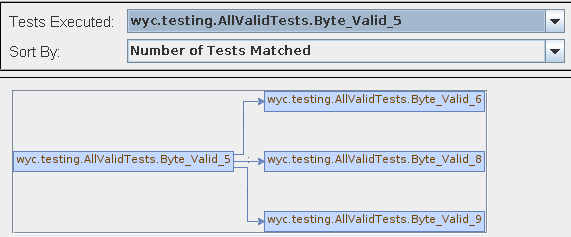
\includegraphics[width=\textwidth]{model24.png}
\end{figure}

This requires further examination of the test cases. This involves examining the Whiley files which would give insight into how closely related these two tests are. Comparing Byte\_Valid\_5 and Byte\_Valid\_8 in figures \ref{fig:byte8} and \ref{fig:byte5} respectively. It shows that the difference between the tests is the range of j and two additional addition statements. The decision whether these two tests are redundant is up to a developer. But there is a possibility that they could be separated or merged to create a single test case.

\begin{figure}[h]
\caption{Byte\_Valid\_8}
\begin{lstlisting}
public method main(System.Console sys) -> void:
    for i in constants:
        for j in 0 .. 8:
            sys.out.print(Any.toString(i) ++ " << ")
            sys.out.print("1+" ++ Any.toString(j) ++ " = ")
            sys.out.println(Any.toString(i << (1 + j)))
\end{lstlisting}
\label{fig:byte8}
\end{figure}

\begin{figure}[h]
\caption{Byte\_Valid\_5}
\begin{lstlisting}
public method main(System.Console sys) -> void:
    for i in constants:
        for j in 0 .. 9:
            sys.out.print(Any.toString(i) ++ " << ")
            sys.out.print(Any.toString(j) ++ " = ")
            sys.out.println(Any.toString(i << j))
\end{lstlisting}
\label{fig:byte5}
\end{figure}